% ============================================================
%  Main_Body.tex  –  Game Tracker
% ============================================================

\chapter{Desarrollo}

En este capítulo se describe la implementación técnica del sistema \textit{Game Tracker}. El desarrollo se basó en principios de diseño sólido (SOLID) y una arquitectura orientada a servicios, asegurando que la aplicación sea escalable, segura y fácil de mantener.

% ════════════════════════════════════════════════════════════
\section{Arquitectura del Sistema}
% ════════════════════════════════════════════════════════════

El sistema utiliza una arquitectura de \textbf{N-Capas} con un desacoplamiento total entre el cliente (Frontend) y el servidor (Backend).

\subsection{Modelo Cliente-Servidor}

Game Tracker sigue una arquitectura \textbf{cliente-servidor}, en la que dos
componentes bien diferenciados se comunican a través de una API REST sin
conocer los detalles internos del otro. Esta separación permite que ambas partes
evolucionen de forma independiente: se puede cambiar la interfaz móvil sin tocar
el servidor, y actualizar la lógica del backend sin afectar a la aplicación.

\begin{itemize}
    \item \textbf{Servidor (Backend)}: aplicación Java construida con Spring
    Boot. Expone una API REST sobre HTTPS, gestiona la lógica de negocio,
    aplica las reglas de autorización por roles y persiste los datos en una
    base de datos MySQL administrada en la nube a través de Aiven. El servidor
    se despliega en Render y es completamente \textit{sin estado}: no guarda
    sesiones entre peticiones, ya que toda la autenticación se delega a
    tokens JWT.

    \item \textbf{Cliente (Frontend)}: aplicación móvil desarrollada en
    Flutter. Se encarga exclusivamente de presentar la información al usuario,
    recibir sus acciones y traducirlas en peticiones HTTP hacia el backend.
    El cliente almacena el token JWT localmente mediante
    \texttt{SharedPreferences} para mantener la sesión activa entre usos.
\end{itemize}

% FIX: <-> envuelto en {<->} para evitar conflicto con babel/polyglossia
\begin{figure}[H]
    \centering
    \begin{tikzpicture}[
        node distance=2.5cm,
        >=Stealth,
        block/.style={rectangle, draw=AquaAccent, thick, fill=BoxBg,
            text=TextPrimary, text width=3cm, align=center,
            minimum height=1.2cm, rounded corners=2pt, font=\small\bfseries},
        database/.style={cylinder, draw=AquaAccent, thick, fill=BoxBg,
            text=TextPrimary, shape border rotate=90, minimum width=1.8cm,
            minimum height=2cm, text width=1.5cm, align=center, font=\small\bfseries},
        label/.style={font=\tiny\ttfamily, color=HeadingGray}
    ]
    \node [block] (frontend) {FRONTEND \\ (Flutter)};
    \node [block, right=of frontend] (backend) {BACKEND \\ (Spring Boot)};
    \node [database, right=of backend] (db) {DB \\ (MySQL)};
    \draw [thick, AquaAccent, {<->}] (frontend) -- node[above, label] {REST/JSON} (backend);
    \draw [thick, AquaAccent, {<->}] (backend) -- node[above, label] {JPA} (db);
    \end{tikzpicture}
    \caption{Arquitectura General del Sistema}
\end{figure}

\subsection{Flujo General de una Petición}

El ciclo de vida de una operación típica en Game Tracker, como agregar una
nota a un juego, sigue estos pasos:

\begin{enumerate}
    \item El usuario escribe su nota en la interfaz de Flutter y presiona
    el botón de enviar.
    \item El servicio HTTP del cliente adjunta el token JWT en el encabezado
    \texttt{Authorization} y envía una petición \texttt{POST} al endpoint
    \texttt{/api/juegos/\{id\}/notes}.
    \item El filtro \texttt{AuthTokenFilter} del backend intercepta la petición,
    valida el token y carga el contexto de seguridad con los datos del usuario.
    \item \texttt{GameController} recibe la petición, verifica que el contenido
    no esté vacío, asocia la nota al usuario autenticado y delega el guardado
    al repositorio JPA.
    \item La base de datos MySQL persiste la nueva nota y el servidor devuelve
    la entidad actualizada en formato JSON.
    \item Flutter recibe la respuesta, actualiza el estado local y vuelve a
    renderizar la pantalla con la nueva nota visible.
\end{enumerate}

\subsection{Capas del Backend}

Internamente, el servidor organiza su código en capas con responsabilidades
bien definidas:

\begin{itemize}
    \item \textbf{Controladores}: reciben las peticiones HTTP, validan los
    parámetros básicos y delegan el trabajo a los servicios o repositorios
    correspondientes. Ejemplos: \texttt{GameController},
    \texttt{AuthController}, \texttt{ReactionController}.

    \item \textbf{Servicios}: contienen la lógica de negocio que no pertenece
    directamente a un controlador. Ejemplos: \texttt{GameNoteService} (valida
    el estado de una nota), \texttt{NoteAuthorizationService} (centraliza las
    reglas de permisos) y \texttt{NoteReactionService} (gestiona el ciclo de
    vida de las reacciones).

    \item \textbf{Modelos y entidades}: clases Java anotadas con
    \texttt{@Entity} que Hibernate mapea directamente a tablas MySQL. Las
    entidades principales son \texttt{Game}, \texttt{GameNote}, \texttt{User},
    \texttt{Reaction} y \texttt{NoteReaction}.

    \item \textbf{Repositorios}: interfaces que extienden
    \texttt{JpaRepository} y proveen acceso a la base de datos sin necesidad
    de escribir SQL. Spring Data JPA genera las implementaciones
    automáticamente a partir del nombre de los métodos.

    \item \textbf{Seguridad}: paquete que contiene el filtro JWT
    (\texttt{AuthTokenFilter}), la configuración de Spring Security
    (\texttt{WebSecurityConfig}) y los servicios de usuario necesarios para
    la autenticación (\texttt{UserDetailsServiceImpl}).
\end{itemize}

\subsection{Esquema de la Base de Datos}

Las tablas principales que sostienen la lógica del sistema son:

\begin{itemize}
    \item \texttt{juegos}: almacena el catálogo de videojuegos con sus
    atributos —nombre, franquicia, categoría, calificación, estado de progreso
    y URL de portada—.
    \item \texttt{notes}: guarda las notas y comentarios asociados a cada
    juego, incluyendo autor, fecha y un indicador de borrado lógico.
    \item \texttt{users} y \texttt{roles}: gestionan las cuentas de usuario
    y sus niveles de acceso (usuario, moderador y administrador).
    \item \texttt{reactions} y \texttt{note\_reactions}: catálogo de tipos de
    reacción disponibles y registro de qué usuario reaccionó a qué nota.
\end{itemize}

% ════════════════════════════════════════════════════════════
\section{Patrones de Diseño}
% ════════════════════════════════════════════════════════════

Un patrón de diseño es una solución reutilizable a un problema que aparece con
frecuencia durante el desarrollo de software. No son fragmentos de código que
se copian directamente, sino plantillas que describen cómo estructurar clases
y objetos para resolver un problema de forma ordenada. En Game Tracker se
aplicaron cuatro patrones de manera deliberada y justificada.

% ────────────────────────────────────────────────────────────
\subsection{MVC — Modelo Vista Controlador}
% ────────────────────────────────────────────────────────────

\begin{patternbox}{Patrón Arquitectural}{MVC — Modelo Vista Controlador}

\textbf{¿Qué es?}

MVC divide una aplicación en tres capas con responsabilidades claramente
separadas. El \textbf{Modelo} representa los datos y las reglas de negocio.
La \textbf{Vista} se encarga de mostrar la información al usuario. El
\textbf{Controlador} actúa como intermediario: recibe las acciones del usuario,
interactúa con el modelo y decide qué respuesta devolver. El objetivo es que
ninguna de las tres capas conozca los detalles internos de las otras dos.

\vspace{0.5em}
\textbf{¿Cómo funciona en Game Tracker?}

El patrón se aplica en dos niveles simultáneos dentro del proyecto:

\begin{itemize}
    \item \textbf{Backend (Spring Boot)}: las clases \texttt{@Entity}
    —como \texttt{Game} y \texttt{GameNote}— son el \textbf{Modelo}, ya que
    representan los datos que se persisten en MySQL. Las clases
    \texttt{@RestController} —como \texttt{GameController} y
    \texttt{AuthController}— son los \textbf{Controladores}: reciben las
    peticiones HTTP y coordinan la respuesta. El JSON que devuelve la API
    hacia Flutter representa la \textbf{Vista}: la capa de presentación que
    consume el cliente.

    \item \textbf{Frontend (Flutter)}: los widgets de la aplicación actúan
    como la \textbf{Vista} que el usuario ve. Los servicios HTTP
    (\texttt{ApiService}, \texttt{AuthService}) gestionan el acceso a los
    datos (\textbf{Modelo}). Los controladores como
    \texttt{ReactionTimelineController} coordinan la lógica entre ambos.
\end{itemize}

Por ejemplo, cuando un usuario edita un juego, Flutter (Vista) envía una
petición \texttt{PUT}. \texttt{GameController} (Controlador) la recibe,
actualiza los campos del objeto \texttt{Game} (Modelo) y persiste el cambio
mediante el repositorio JPA.

\vspace{0.5em}
\textbf{¿Por qué lo elegí?}

Spring Boot impone MVC de forma natural a través de sus anotaciones. La
alternativa directa sería un enfoque de \textit{Transaction Script}, en el que
toda la lógica vive dentro del controlador. Ese estilo es funcional para
proyectos pequeños, pero no escala cuando las reglas de negocio crecen. MVC
garantiza que se pueda modificar la presentación de la API sin tocar los
modelos, y agregar nuevos modelos sin modificar los controladores existentes.

\end{patternbox}

% ────────────────────────────────────────────────────────────
\subsection{Singleton — AuthService en Flutter}
% ────────────────────────────────────────────────────────────

\begin{patternbox}{Patrón Creacional}{Singleton}

\textbf{¿Qué es?}

El Singleton garantiza que una clase tenga \textbf{una única instancia} en
toda la ejecución de la aplicación y proporciona un punto de acceso global a
ella. Se logra haciendo privado el constructor de la clase y exponiendo una
referencia estática a la instancia única.

\vspace{0.5em}
\textbf{¿Cómo funciona en Game Tracker?}

En Flutter, la clase \texttt{AuthService} implementa el Singleton de forma
explícita. Declara una instancia estática privada (\texttt{\_instance}), un
constructor privado nombrado (\texttt{AuthService.\_internal()}) y un
\texttt{factory constructor} que siempre devuelve la misma instancia:

\begin{lstlisting}[language=Dart]
class AuthService {
  // Instancia estatica unica -- se crea una sola vez
  static final AuthService _instance = AuthService._internal();

  // Constructor privado: nadie puede crear una segunda instancia
  AuthService._internal() {
    _httpClient = http.Client();
  }

  // Cualquier llamada a AuthService() devuelve la misma instancia
  factory AuthService() => _instance;
}
\end{lstlisting}

\texttt{AuthService} gestiona el token JWT, las credenciales del usuario y el
estado de sesión. Al ser Singleton, cualquier pantalla de la aplicación que
invoque \texttt{AuthService()} obtiene exactamente el mismo objeto con el
mismo token cargado, sin necesidad de pasarlo como parámetro entre pantallas.

\vspace{0.5em}
\textbf{¿Por qué este patrón?}

El token JWT y los datos del usuario autenticado son información que múltiples
partes de la aplicación necesitan: la pantalla de inicio, el formulario de
edición de un juego, el módulo de notas, etc. Si \texttt{AuthService} no fuera
Singleton, cada componente crearía su propia instancia con su propio estado de
sesión, lo que generaría inconsistencias. La alternativa más común sería
inyectar el token manualmente como argumento a través del árbol de widgets,
pero eso ensucia las firmas de cada clase con información que no le pertenece.
Singleton mantiene la coherencia de sesión de forma transparente.

\subsection{Evidencias de Código: Singleton (AuthService)}

\begin{figure}[H]
    \centering
    % FILA 1: Inicio y Constructor privado
    \begin{minipage}{0.45\textwidth}
        \centering
        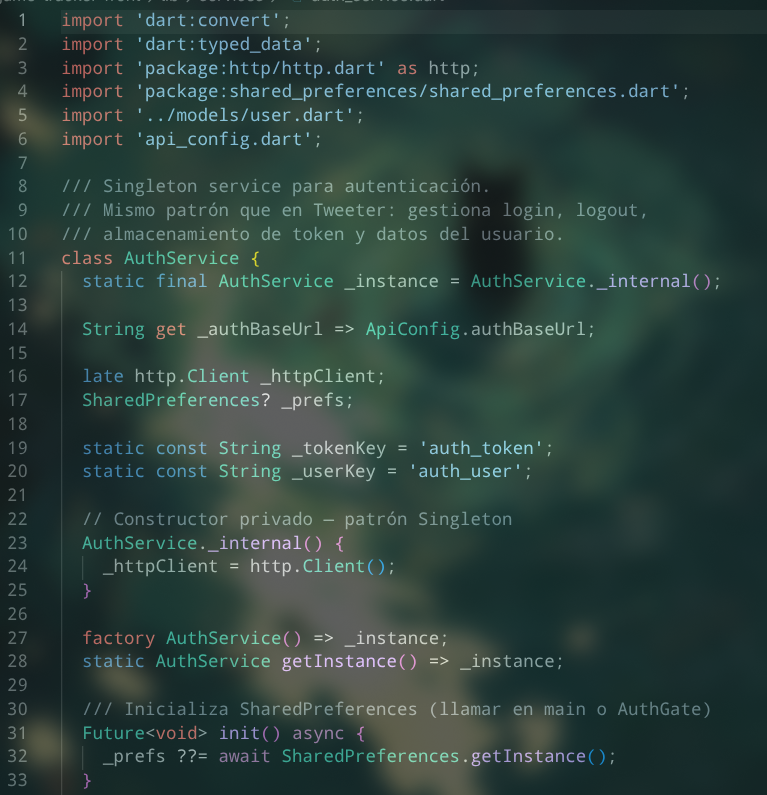
\includegraphics[width=\textwidth]{Resources/Singleton/Singleton-1.png}
        \caption*{Parte 1: Instancia estática}
    \end{minipage}
    \hfill
    \begin{minipage}{0.45\textwidth}
        \centering
        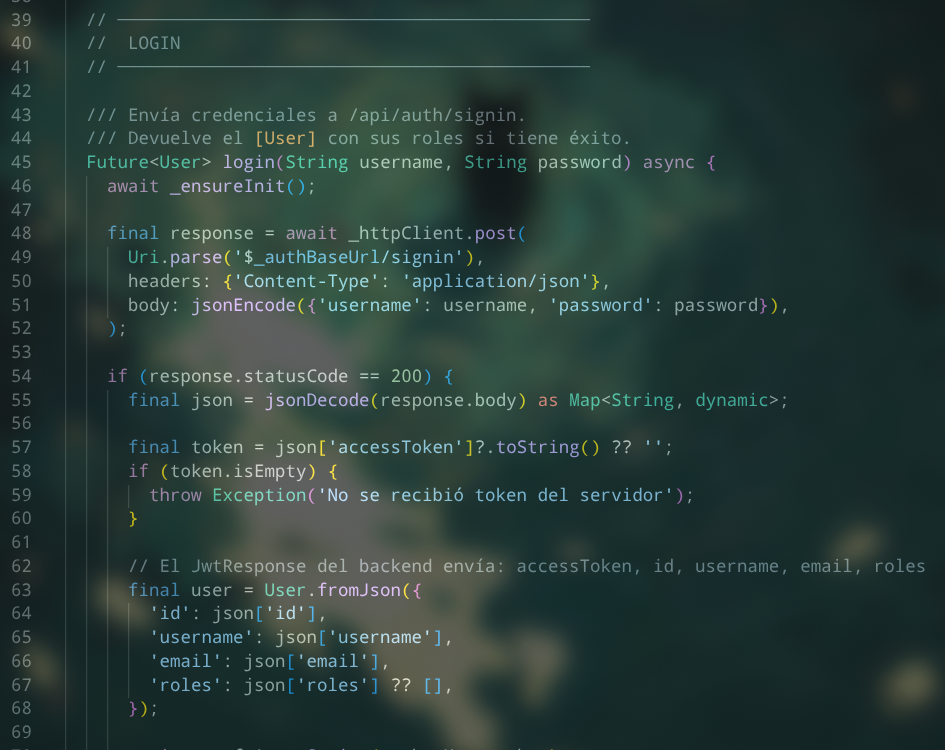
\includegraphics[width=\textwidth]{Resources/Singleton/Singleton-2.png}
        \caption*{Parte 2: Constructor privado}
    \end{minipage}

    \vspace{2em}

    % FILA 2: Métodos de acceso y estado
    \begin{minipage}{0.45\textwidth}
        \centering
        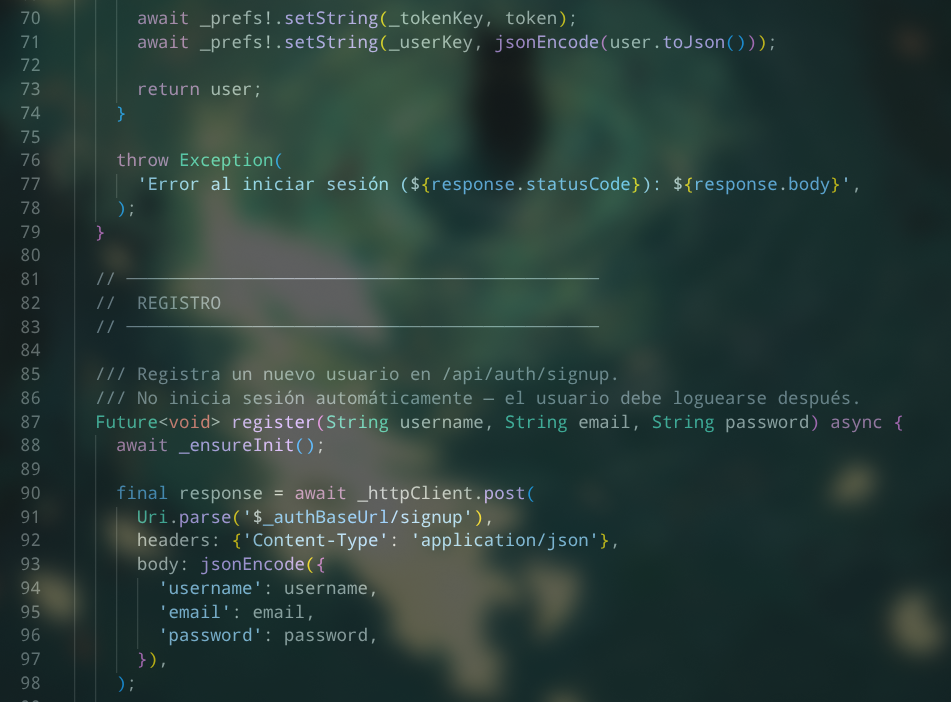
\includegraphics[width=\textwidth]{Resources/Singleton/Singleton-3.png}
        \caption*{Parte 3: Acceso a la instancia}
    \end{minipage}
    \hfill
    \begin{minipage}{0.45\textwidth}
        \centering
        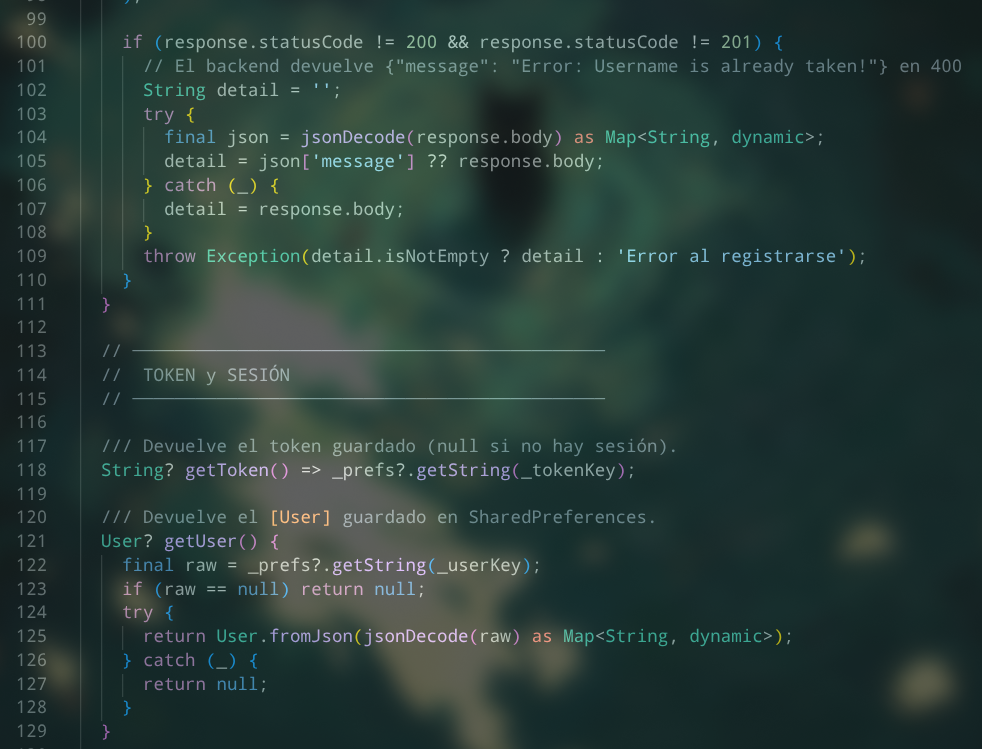
\includegraphics[width=\textwidth]{Resources/Singleton/Singleton-4.png}
        \caption*{Parte 4: Manejo de sesión}
    \end{minipage}

    \vspace{2em}

    % FILA 3: Persistencia y Token
    \begin{minipage}{0.45\textwidth}
        \centering
        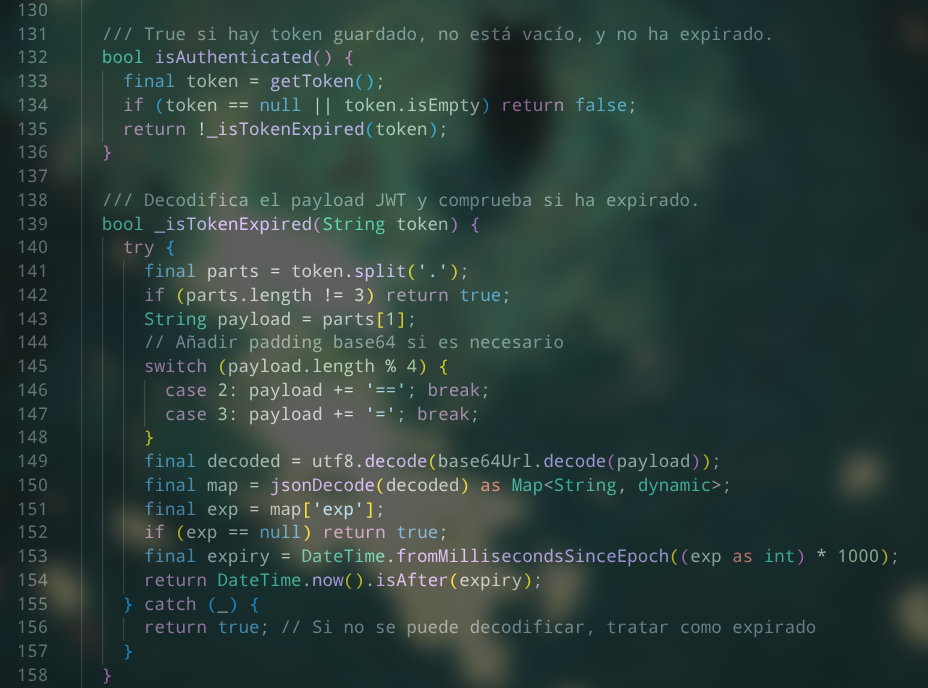
\includegraphics[width=\textwidth]{Resources/Singleton/Singleton-5.png}
        \caption*{Parte 5: Persistencia de datos}
    \end{minipage}
    \hfill
    \begin{minipage}{0.45\textwidth}
        \centering
        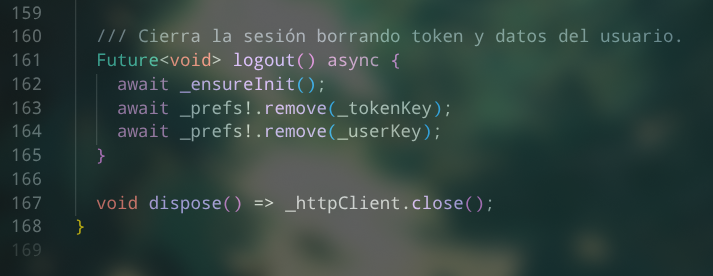
\includegraphics[width=\textwidth]{Resources/Singleton/Singleton-6.png}
        \caption*{Parte 6: Recuperación del Token}
    \end{minipage}

    \vspace{1.5em}
    \caption{Implementación del patrón Singleton para la gestión de autenticación.}
\end{figure}

\end{patternbox}

% ────────────────────────────────────────────────────────────
\subsection{Strategy — Conteo y Eliminación de Notas}
% ────────────────────────────────────────────────────────────

\begin{patternbox}{Patrón de Comportamiento}{Strategy}

\textbf{¿Qué es?}

El patrón Strategy define una \textbf{familia de algoritmos intercambiables},
los encapsula en clases separadas y permite seleccionar cuál usar en tiempo
de ejecución sin modificar el código que los invoca. El componente que usa la
estrategia solo conoce la interfaz común; no le importa qué implementación
concreta está activa.

\vspace{0.5em}
\textbf{¿Cómo funciona en Game Tracker?}

El patrón Strategy se aplicó en dos partes del backend:

\textbf{1.\ Conteo de reacciones} --- se definió la interfaz
\texttt{ReactionSummaryStrategy} con un único método responsable de
contabilizar los tipos de reacción de una lista:

\begin{lstlisting}[language=Java]
public interface ReactionSummaryStrategy {
    // Recibe las reacciones y devuelve un mapa {"FUNNY": 5, "SAD": 1}
    Map<String, Long> countReactions(List<NoteReaction> reactions);
}
\end{lstlisting}

La implementación concreta \texttt{EnumReactionSummaryStrategy} utiliza un
\texttt{EnumMap} para recorrer la lista en un único paso (complejidad O(n)).
Si en el futuro se requiere una estrategia diferente —por ejemplo, una que
excluya reacciones de cuentas baneadas— basta con crear una nueva clase que
implemente la misma interfaz, sin modificar ningún controlador.

\textbf{2.\ Estrategia de eliminación de notas} --- las notas de un juego
pueden eliminarse de tres formas distintas según el rol del usuario:

\begin{itemize}
    \item \texttt{SOFT\_DELETE}: marca la nota como eliminada y reemplaza el
    contenido con un texto indicativo. Preserva la estructura del hilo de
    respuestas. Disponible para autores, moderadores y administradores.
    \item \texttt{HARD\_DELETE}: borra físicamente la nota de la base de datos.
    Solo permitido si la nota no tiene respuestas. Disponible para autores,
    moderadores y administradores.
    \item \texttt{CASCADE\_DELETE}: elimina la nota y todas sus respuestas de
    forma recursiva. Exclusivo para administradores.
\end{itemize}

\texttt{GameController} selecciona la estrategia según el parámetro
\texttt{?strategy=} de la petición y ejecuta la lógica correspondiente sin
que el llamante necesite conocer los detalles de ninguna de las tres variantes.

\vspace{0.5em}
\textbf{¿Por qué lo elegí?}

La alternativa directa era una cadena de \texttt{if-else} dentro del
controlador. Eso funciona para dos casos, pero al incorporar la tercera
variante (\texttt{CASCADE\_DELETE}) el método empezó a crecer de forma
difícil de mantener. Strategy permite agregar nuevas formas de eliminación sin
modificar la lógica existente, siguiendo el principio Open/Closed. Se consideró
el patrón Command, pero habría añadido complejidad innecesaria para un problema
que se resuelve limpiamente con una interfaz y tres implementaciones.

\subsection{Evidencias de Código: Strategy (Patrones de Borrado)}

% --- PRIMERA PARTE: La Interfaz y la Estrategia 1 ---
\begin{figure}[H]
    \centering
    \begin{minipage}{0.48\textwidth}
        \centering
        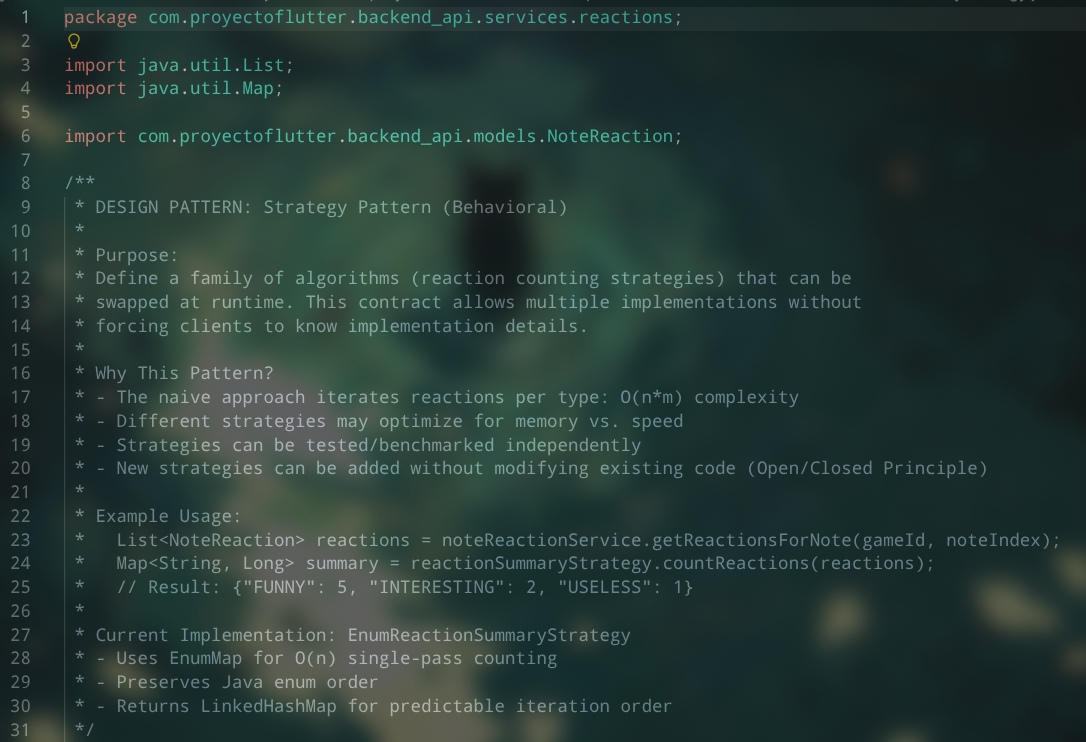
\includegraphics[width=\textwidth]{Resources/Strategy/Strategy-1.1.png}
        \caption*{Parte 1: Interfaz \texttt{DeleteStrategy}}
    \end{minipage}
    \hfill
    \begin{minipage}{0.48\textwidth}
        \centering
        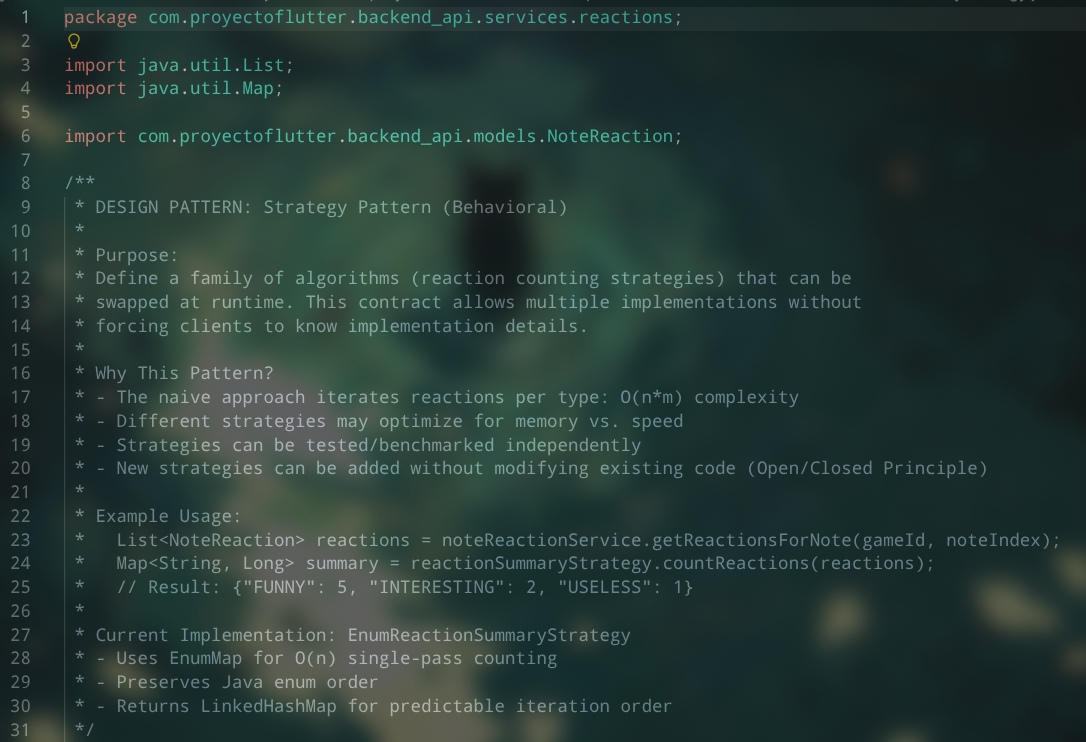
\includegraphics[width=\textwidth]{Resources/Strategy/Strategy-1.1.png}
        \caption*{Parte 2: Implementación \texttt{PhysicalDelete}}
    \end{minipage}
    
    \vspace{2em}
    \caption{Definición de la interfaz y primera estrategia de eliminación.}
\end{figure}

% --- SEGUNDA PARTE: La Estrategia 2 (Destacada) ---
\begin{figure}[H]
    \centering
    \begin{minipage}{0.7\textwidth} % Más grande para resaltar la lógica compleja
        \centering
        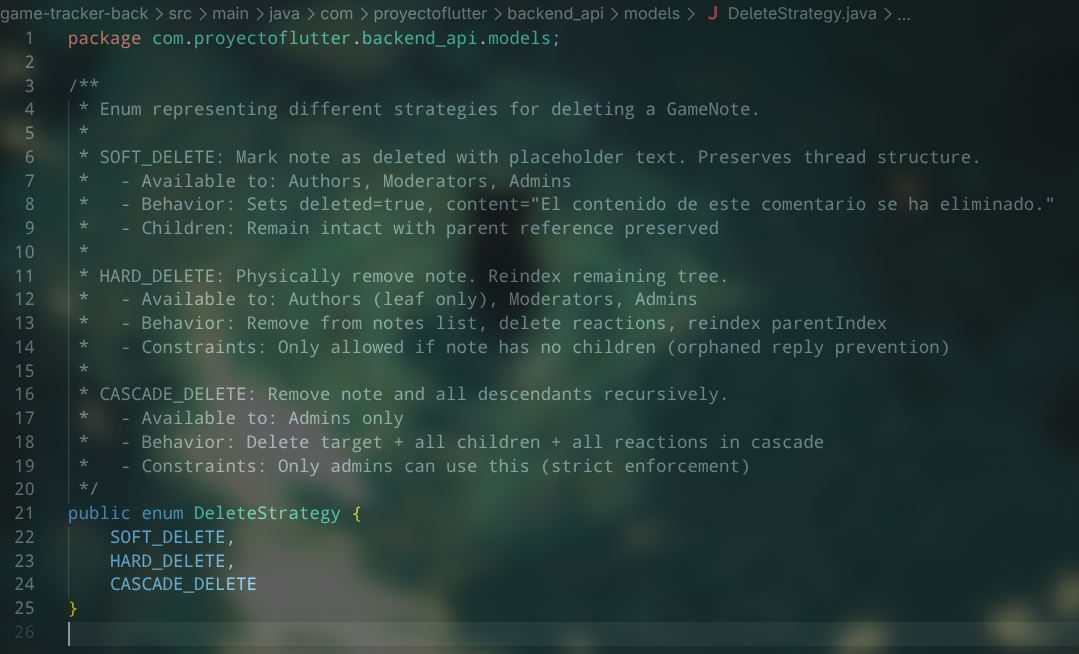
\includegraphics[width=\textwidth]{Resources/Strategy/Strategy-2.png}
        \caption*{Parte 3: Implementación \texttt{SoftDelete} (Borrado Lógico)}
    \end{minipage}
    
    \vspace{1.5em}
    \caption{Segunda estrategia de eliminación implementando el patrón Strategy.}
\end{figure}

\end{patternbox}

% ────────────────────────────────────────────────────────────
\subsection{ChangeNotifier — Gestión de Estado en Flutter}
% ────────────────────────────────────────────────────────────

\begin{patternbox}{Patrón de Comportamiento / Gestión de Estado}{ChangeNotifier}

\textbf{¿Qué es?}

\texttt{ChangeNotifier} es la solución nativa de Flutter para gestionar estado.
Una clase que extiende \texttt{ChangeNotifier} puede notificar a sus
observadores cada vez que su estado interno cambia, invocando
\texttt{notifyListeners()}. Los widgets que escuchan al notificador se
reconstruyen automáticamente para reflejar el nuevo estado. Este patrón
combina las ideas del \textit{Observer} (notificar cambios) con el
\textit{Controlador} de MVC (separar lógica de la vista).

\vspace{0.5em}
\textbf{¿Cómo funciona en Game Tracker?}

La clase \texttt{ReactionTimelineController} extiende \texttt{ChangeNotifier}
y es responsable de toda la lógica relacionada con las reacciones del usuario
en el modal de un juego. Gestiona los siguientes estados:

\begin{itemize}
    \item \texttt{\_loading}: indica si hay una petición HTTP en curso
    (la interfaz muestra un indicador de progreso).
    \item \texttt{\_loaded}: indica que los datos ya están disponibles
    (la interfaz muestra los botones de reacción con sus conteos).
    \item \texttt{\_error}: contiene el mensaje de error si la petición falló.
    \item \texttt{\_reactionSummaries}: mapa de índice de nota hacia su resumen
    de reacciones, actualizado después de cada interacción del usuario.
\end{itemize}

El ciclo de uso típico es el siguiente: cuando el usuario abre el modal de
reacciones, la pantalla llama a \texttt{controller.prepareForGame(game)} para
limpiar cualquier estado anterior, y luego a \texttt{controller.ensureLoaded(game)}
para cargar los datos. Mientras se cargan, la pantalla muestra un indicador
basándose en \texttt{controller.isLoading}. Una vez listos, los botones de
reacción se renderizan con los conteos actualizados. Si el usuario presiona una
reacción, la pantalla llama a \texttt{controller.toggleReaction(...)} y el modal
se actualiza sin necesidad de recargar toda la pantalla.

\vspace{0.5em}
\textbf{¿Por qué lo elegí?}

La alternativa más simple habría sido usar \texttt{setState} directamente dentro
del widget de la pantalla. Sin embargo, eso mezcla la lógica de negocio
—llamadas HTTP, manejo de errores, reindexado de notas— con el código de la
interfaz, lo que produce widgets muy largos y difíciles de probar. Al extraer
toda esa lógica a un \texttt{ChangeNotifier}, la pantalla se vuelve delgada:
solo decide qué mostrar según el estado que expone el controlador. Se consideró
usar bibliotecas más completas como \textit{Provider} o \textit{Riverpod}, pero
para el alcance del proyecto \texttt{ChangeNotifier} es más que suficiente,
no requiere dependencias adicionales y es la solución recomendada por la
documentación oficial de Flutter para casos de esta escala.


\subsection{Evidencias de Código: ChangeNotifier}

% --- PRIMERA PARTE (4 imágenes) ---
\begin{figure}[H]
    \centering
    \begin{minipage}{0.45\textwidth}
        \centering
        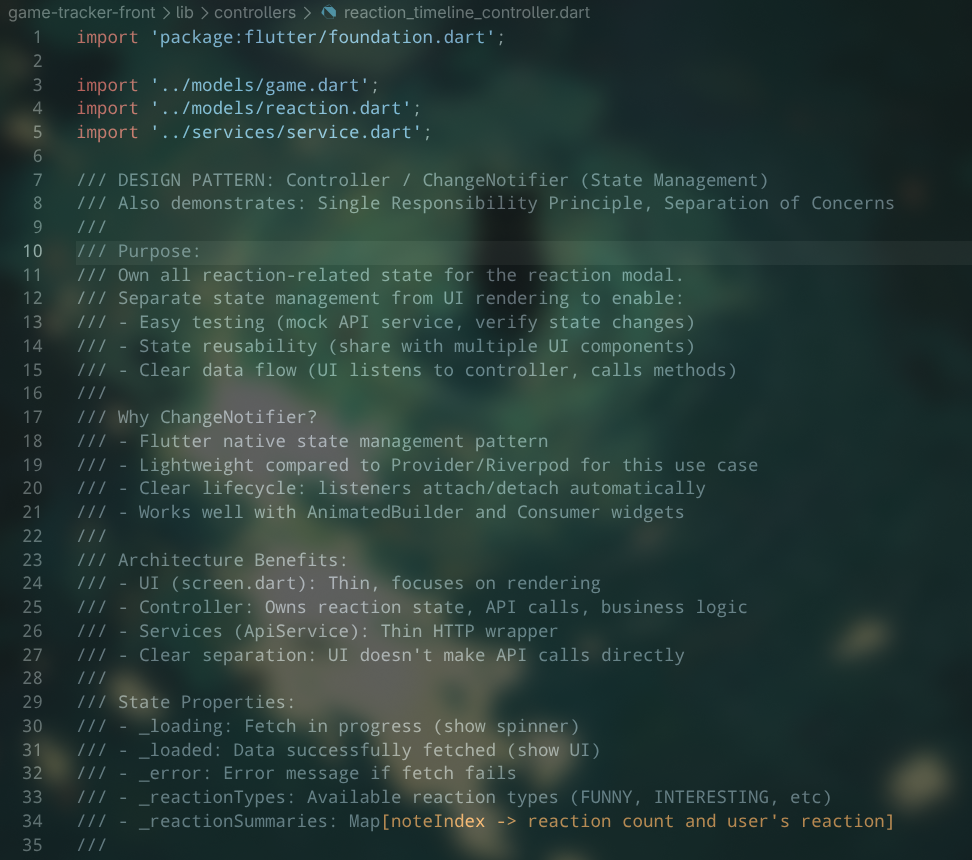
\includegraphics[width=\textwidth]{Resources/ChangeNotifier/ChangeNotifier-1.png}
        \caption*{Parte 1: Definición de la clase}
    \end{minipage}
    \hfill
    \begin{minipage}{0.45\textwidth}
        \centering
        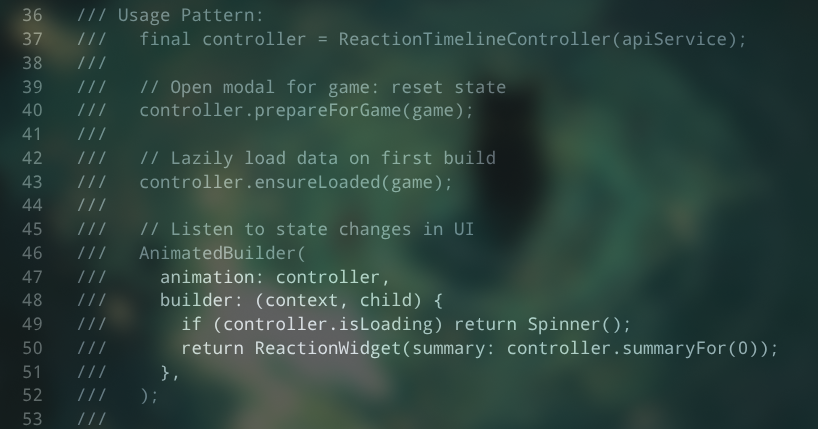
\includegraphics[width=\textwidth]{Resources/ChangeNotifier/ChangeNotifier-2.png}
        \caption*{Parte 2: Variables de estado}
    \end{minipage}

    \vspace{2em}

    \begin{minipage}{0.45\textwidth}
        \centering
        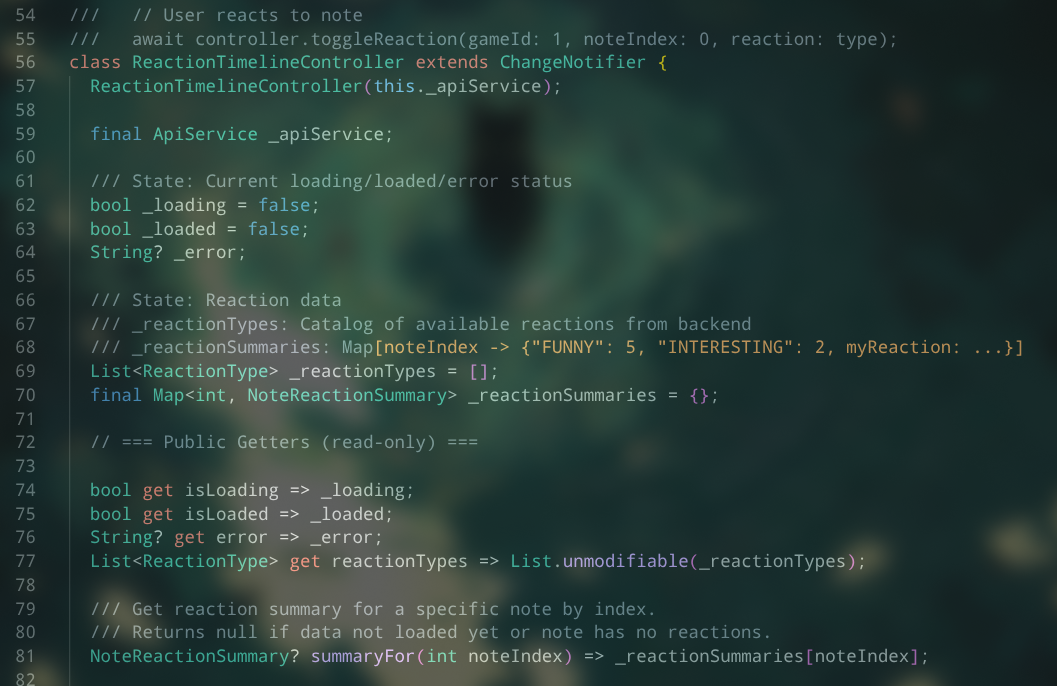
\includegraphics[width=\textwidth]{Resources/ChangeNotifier/ChangeNotifier-3.png}
        \caption*{Parte 3: Getters públicos}
    \end{minipage}
    \hfill
    \begin{minipage}{0.45\textwidth}
        \centering
        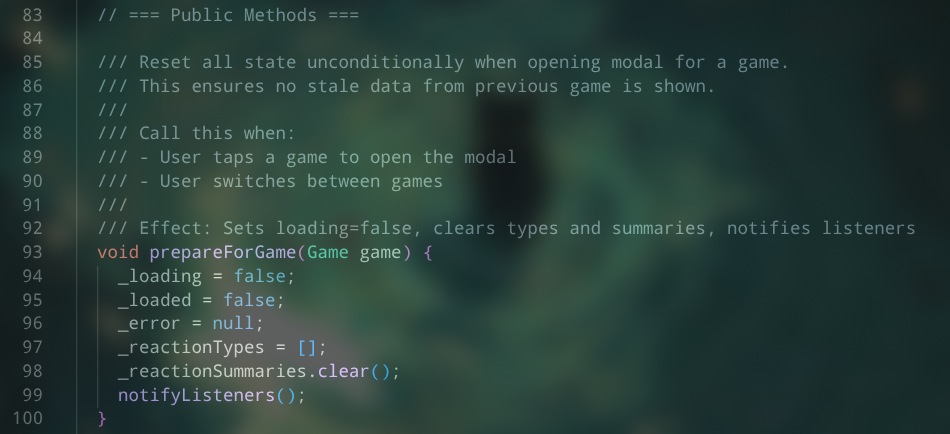
\includegraphics[width=\textwidth]{Resources/ChangeNotifier/ChangeNotifier-4.png}
        \caption*{Parte 4: Método prepareForGame}
    \end{minipage}
    \caption{Implementación del controlador reactivo (1/2).}
\end{figure}

\newpage % Saltamos a la siguiente página para que respiren

% --- SEGUNDA PARTE (Las 5 que faltan) ---
\begin{figure}[H]
    \centering
    \begin{minipage}{0.45\textwidth}
        \centering
        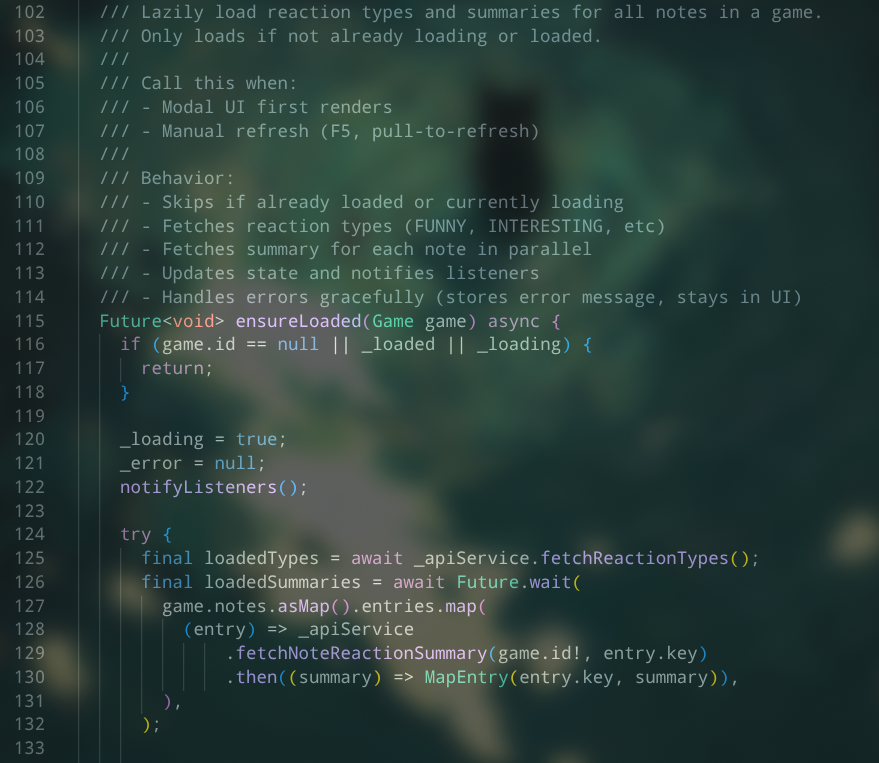
\includegraphics[width=\textwidth]{Resources/ChangeNotifier/ChangeNotifier-5.png}
        \caption*{Parte 5: Lógica de carga}
    \end{minipage}
    \hfill
    \begin{minipage}{0.45\textwidth}
        \centering
        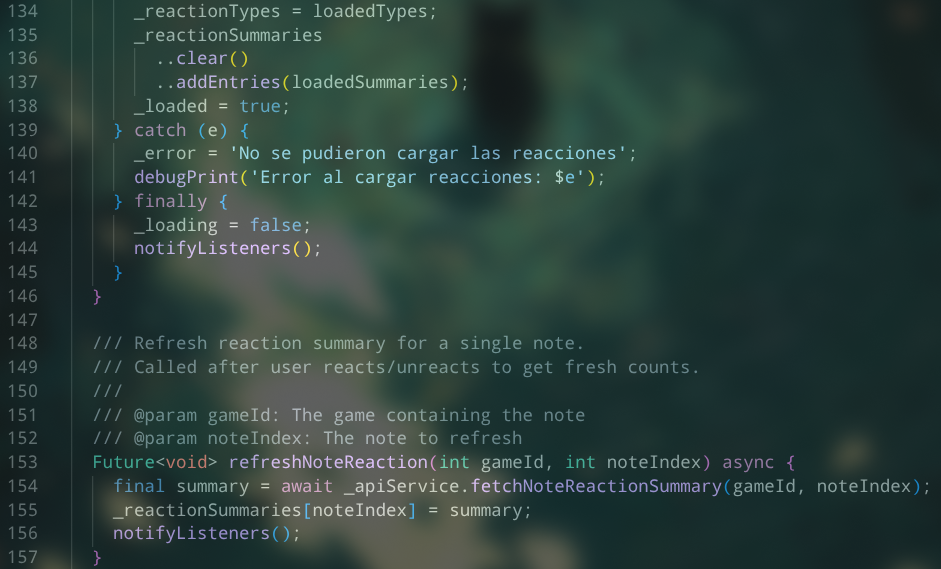
\includegraphics[width=\textwidth]{Resources/ChangeNotifier/ChangeNotifier-6.png}
        \caption*{Parte 6: Manejo de errores}
    \end{minipage}

    \vspace{2em}

    \begin{minipage}{0.45\textwidth}
        \centering
        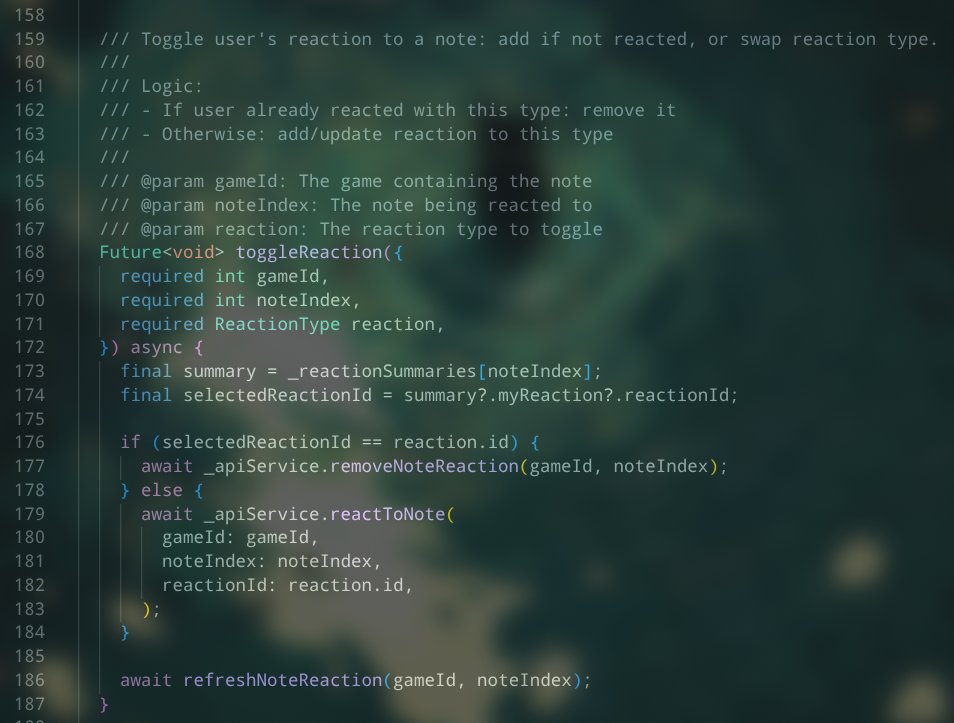
\includegraphics[width=\textwidth]{Resources/ChangeNotifier/ChangeNotifier-7.png}
        \caption*{Parte 7: Toggle de reacciones}
    \end{minipage}
    \hfill
    \begin{minipage}{0.45\textwidth}
        \centering
        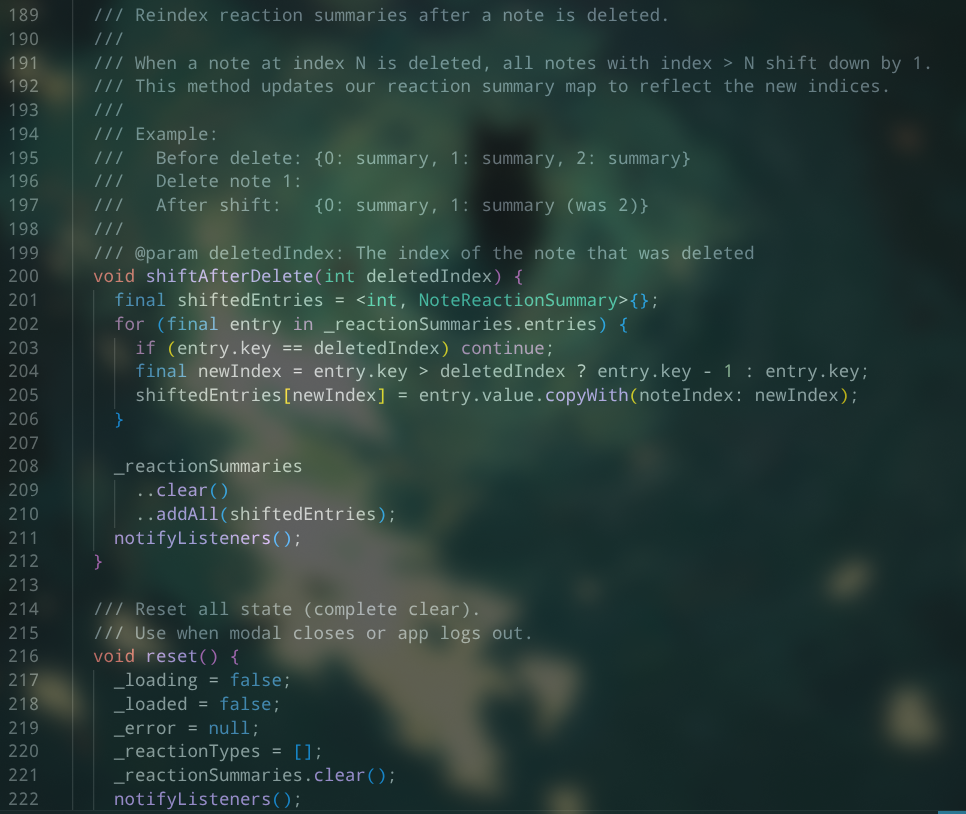
\includegraphics[width=\textwidth]{Resources/ChangeNotifier/ChangeNotifier-8.png}
        \caption*{Parte 8: Shift de índices}
    \end{minipage}

    \vspace{2em}

    \begin{minipage}{0.45\textwidth}
        \centering
        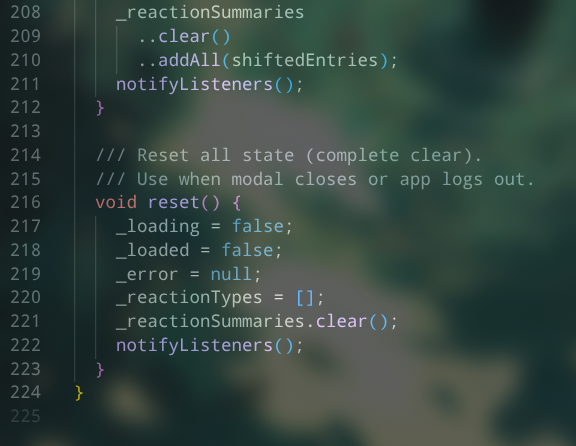
\includegraphics[width=\textwidth]{Resources/ChangeNotifier/ChangeNotifier-9.png}
        \caption*{Parte 9: Reset de estado}
    \end{minipage}
    \caption{Implementación del controlador reactivo (2/2).}
\end{figure}

\end{patternbox}

% ────────────────────────────────────────────────────────────
\subsection{Facade — Simplificación de la Comunicación con la API}
% ────────────────────────────────────────────────────────────

\begin{patternbox}{Patrón Estructural}{Facade (Fachada)}

\textbf{¿Qué es?}

El patrón \textit{Facade} proporciona una interfaz unificada y simplificada para 
un conjunto de interfaces en un subsistema. Actúa como un "punto de entrada" 
que oculta la complejidad del acceso a librerías, protocolos de red o lógicas 
de autenticación, exponiendo únicamente los métodos que el cliente necesita 
realmente utilizar.

\vspace{0.5em}
\textbf{¿Cómo funciona en Game Tracker?}

En el proyecto, la clase \texttt{ReactionApiService} implementa este patrón al 
centralizar todas las operaciones de red relacionadas con las reacciones. En lugar 
de que los controladores o widgets gestionen directamente la librería \texttt{http}, 
la construcción de URLs o el parseo de JSON, simplemente llaman a métodos de alto 
nivel. El servicio se encarga de:

\begin{itemize}
    \item \textbf{Gestión de Cabeceras:} Utiliza internamente el \texttt{AuthService} 
    para inyectar automáticamente el token JWT en el \textit{header} de autorización.
    \item \textbf{Manejo de Endpoints:} Construye dinámicamente las rutas hacia 
    el servidor (ej. \texttt{/notes/reactions/games/\{id\}}) ocultando la estructura 
    del backend.
    \item \textbf{Adaptación de Datos:} Transforma las respuestas crudas de la red 
    en modelos de datos tipados (\texttt{ReactionType}, \texttt{NoteReactionSummary}), 
    actuando también como un adaptador.
\end{itemize}

Un ejemplo claro es el método \texttt{toggleReaction} del controlador, el cual no sabe 
nada sobre protocolos HTTP o tokens de seguridad; solo invoca al \texttt{ApiService} 
y espera la respuesta procesada.

\vspace{0.5em}
\textbf{¿Por qué lo elegí?}

Sin este patrón, cada vez que el backend cambiara la ruta de un \textit{endpoint} 
o la estructura de un objeto JSON, habría que modificar múltiples archivos en el 
frontend. El uso de una \textit{Fachada} permite que el código sea \textbf{DRY} 
(\textit{Don't Repeat Yourself}), centralizando el mantenimiento en un solo lugar. 
Además, facilita la legibilidad: es mucho más claro leer un método llamado 
\texttt{fetchReactionTypes()} que ver diez líneas de código configurando una 
petición \texttt{http.get} con validación de estados y decodificación de bytes. 
Esto asegura que la lógica de comunicación sea independiente de la lógica de 
presentación de la aplicación.

\subsection{Evidencias de Código: Facade (ReactionApiService)}

% --- PRIMERA PARTE (4 imágenes en rejilla 2x2) ---
\begin{figure}[H]
    \centering
    \begin{minipage}{0.45\textwidth}
        \centering
        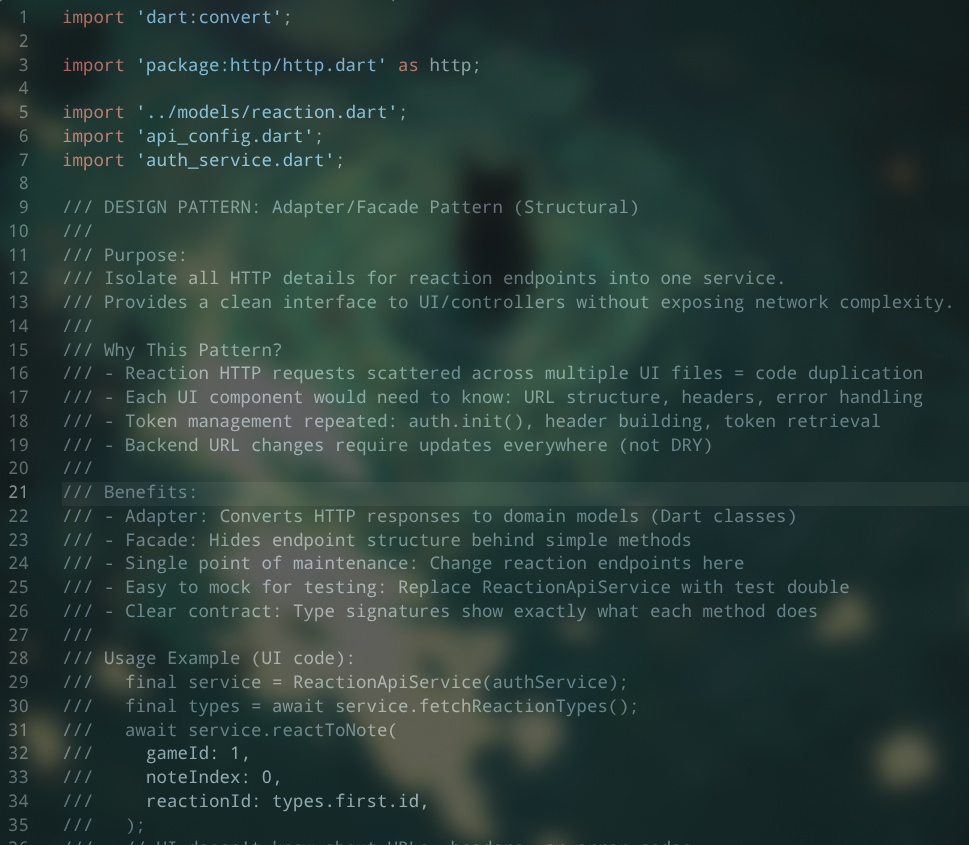
\includegraphics[width=\textwidth]{Resources/Facade/Facade-1.png}
        \caption*{Parte 1: Configuración de Endpoints}
    \end{minipage}
    \hfill
    \begin{minipage}{0.45\textwidth}
        \centering
        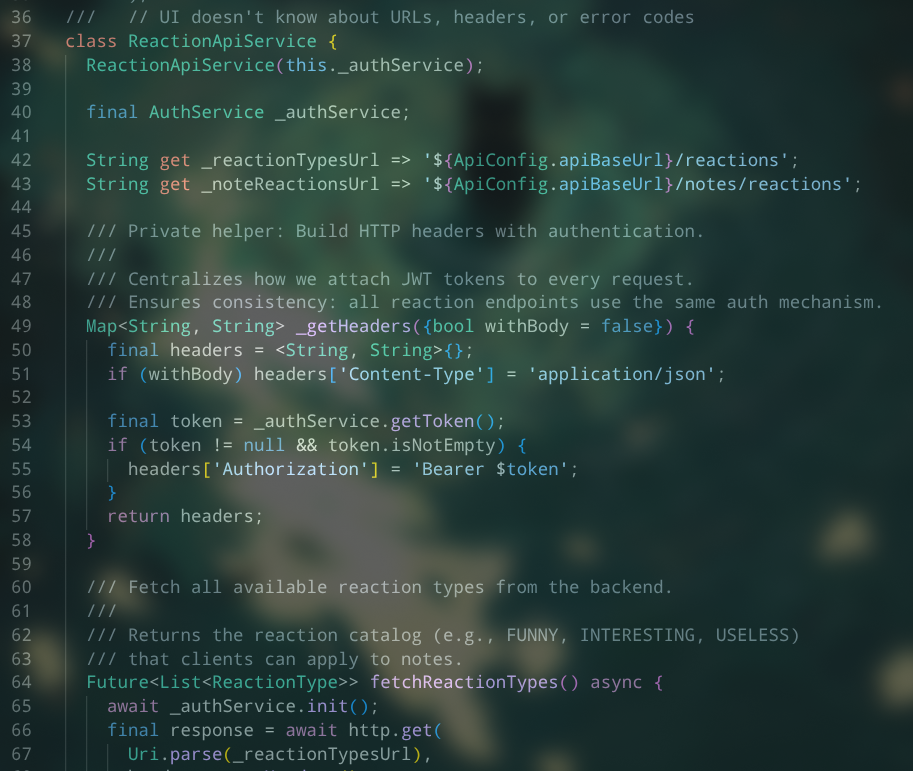
\includegraphics[width=\textwidth]{Resources/Facade/Facade-2.png}
        \caption*{Parte 2: Gestión de Headers y Auth}
    \end{minipage}

    \vspace{2.5em} % Espacio generoso entre filas

    \begin{minipage}{0.45\textwidth}
        \centering
        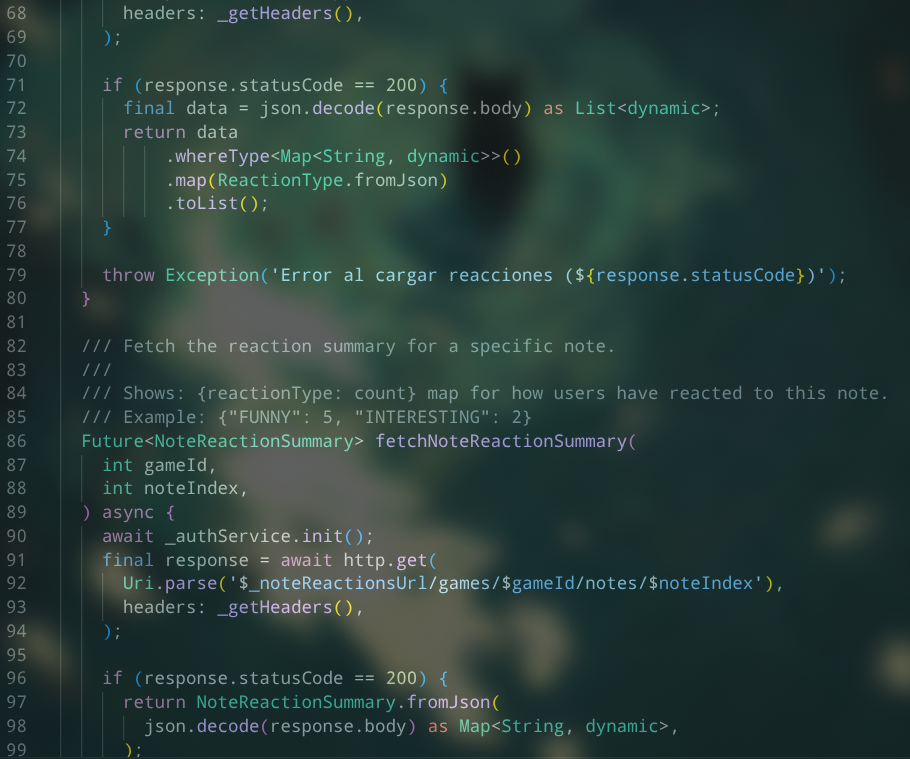
\includegraphics[width=\textwidth]{Resources/Facade/Facade-3.png}
        \caption*{Parte 3: Fetch de Catálogos}
    \end{minipage}
    \hfill
    \begin{minipage}{0.45\textwidth}
        \centering
        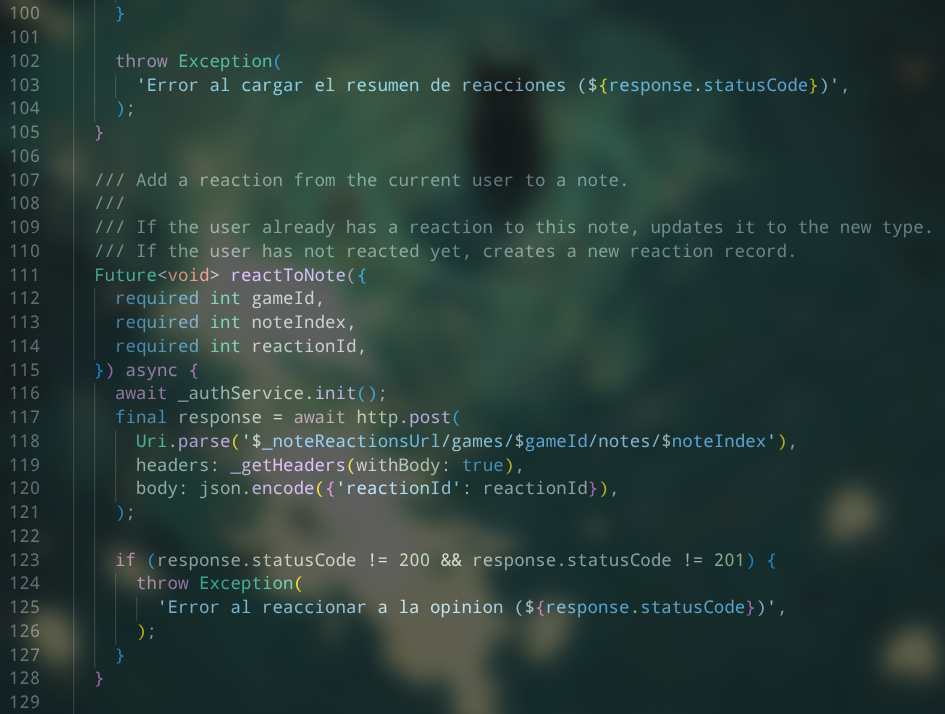
\includegraphics[width=\textwidth]{Resources/Facade/Facade-4.png}
        \caption*{Parte 4: Resumen de Reacciones}
    \end{minipage}
    \caption{Implementación de la Fachada de servicios de red (1/2).}
\end{figure}

\newpage % Salto de página para la última imagen

% --- SEGUNDA PARTE (La imagen 5 centrada y destacada) ---
\begin{figure}[H]
    \centering
    \begin{minipage}{0.6\textwidth} % Un poco más grande por estar sola
        \centering
        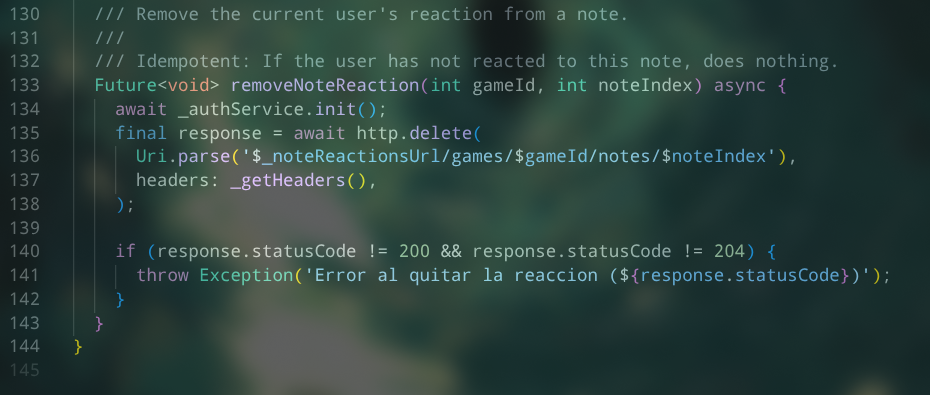
\includegraphics[width=\textwidth]{Resources/Facade/Facade-5.png}
        \caption*{Parte 5: Lógica de Toggle y Delete}
    \end{minipage}
    
    \vspace{1.5em}
    \caption{Implementación de la Fachada de servicios de red (2/2).}
\end{figure}

\end{patternbox}

% ════════════════════════════════════════════════════════════
\section{Modelo de Datos y Persistencia}
% ════════════════════════════════════════════════════════════

Se diseñó un esquema relacional normalizado en MySQL (Aiven). A continuación
se muestra la implementación de las entidades JPA.

\begin{lstlisting}[language=Java, caption=Entidad de Usuario y relaciones]
@Entity
@Table(name = "users")
public class User {
    @Id
    @GeneratedValue(strategy = GenerationType.IDENTITY)
    private Long id;

    @Column(unique = true, nullable = false)
    private String username;

    @OneToMany(mappedBy = "user", cascade = CascadeType.ALL)
    private List<Game> library;
}
\end{lstlisting}

% ════════════════════════════════════════════════════════════
\section{Seguridad: Autenticación con JWT}
% ════════════════════════════════════════════════════════════

La autenticación en Game Tracker se basa en \textbf{JSON Web Tokens (JWT)},
un estándar que permite transmitir información verificable entre cliente y
servidor de forma compacta y sin estado de sesión.

Cuando el usuario inicia sesión correctamente, el backend genera un token
firmado con una clave secreta que incluye el nombre de usuario, sus roles y
una fecha de expiración. Este token se devuelve al cliente, que lo almacena
localmente y lo adjunta en el encabezado \texttt{Authorization: Bearer} de
cada petición posterior.

En el lado del servidor, el componente \texttt{AuthTokenFilter} intercepta cada
petición entrante, valida la firma del token mediante \texttt{JwtUtils} y carga
el contexto de seguridad de Spring antes de que la petición llegue al
controlador. Si el token no es válido o ha expirado, el sistema responde de
forma automática con un error 401.

Este diseño sin estado es la razón por la que el servidor no necesita almacenar
sesiones en base de datos: toda la información necesaria para autenticar al
usuario viaja dentro del propio token.

% ════════════════════════════════════════════════════════════
\section{Sistema de Roles y Permisos}
% ════════════════════════════════════════════════════════════

Game Tracker implementa tres niveles de acceso cuyas reglas se aplican de
forma centralizada en \texttt{NoteAuthorizationService}:

\begin{itemize}
    \item \textbf{Usuario (\texttt{ROLE\_USER})}: puede leer el catálogo
    completo sin autenticarse y, con cuenta activa, puede escribir, editar y
    eliminar sus propias notas.
    \item \textbf{Moderador (\texttt{ROLE\_MODERATOR})}: tiene las mismas
    capacidades que un usuario más la posibilidad de eliminar notas de otros
    mediante \texttt{SOFT\_DELETE} o \texttt{HARD\_DELETE}.
    \item \textbf{Administrador (\texttt{ROLE\_ADMIN})}: control total sobre
    el catálogo —crear, editar y eliminar juegos— y el único rol que puede
    ejecutar \texttt{CASCADE\_DELETE} para eliminar una nota junto con todas
    sus respuestas.
\end{itemize}

Centralizar estas reglas en un único servicio evita que la lógica de permisos
quede duplicada o dispersa a través de múltiples controladores, lo que
simplifica tanto el mantenimiento como las pruebas unitarias.

% ════════════════════════════════════════════════════════════
\section{Conclusión del Desarrollo}
% ════════════════════════════════════════════════════════════

La combinación de estos patrones permitió que el proyecto pasara de ser un
simple prototipo a un sistema de nivel profesional. El uso del patrón Strategy
en el backend y ChangeNotifier en el frontend asegura que la experiencia del
usuario sea fluida y la del desarrollador sea organizada.